% =============================================================================
% Chapter 17 — Transplants, Four Sparks, and the Open Lab (closes Part II
% and the book; the appendix and CTA follow)
% =============================================================================

\chapter{Transplants, Four Sparks, and the Open Lab}
\label{ch:transplants}

The published refusal-direction vectors for abliterating GLM-5.3-Flash ---
surgically removing the model's refusal behavior by editing its weights ---
are mathematically sound and, on this model, empirically useless. Measured
against stock \code{o_proj}, their maximum projection
$\lvert r^{\top}W\rvert$ was $0.084$ --- what the overlay's own tests record
as random-unit-vector level.
The publisher's own projection variants top out at 9/32 on their
refusal-bypass gate, a 32-prompt suite scoring how many refusals the edit
actually removes; byte-copying a donor's weights scores 32/32. The lab
measured that rather than assuming it, and the measurement is why the GLM
recipe's weight-editing pipeline is a byte transplant governed by a sha256
manifest rather than an elegant orthogonalization.

That pipeline is the first of this closing chapter's three subjects, and
none of them has a counterpart anywhere in Part I. \emph{Editing a
model's weights at load time} --- not patching Python, not swapping a
checkpoint, but rewriting specific tensors in memory, on both TP ranks,
between weight load and CUDA-graph capture, with the on-disk artifact
untouched --- is a capability the DeepSeek deployment never needed. The
second is the honest version of a question \Cref{ch:scaling} answered with
measurements: what does this lab publish when it wants to support hardware
it does not own? The third is the thing the whole book has been quietly
demonstrating without ever naming: the lab itself runs in public, and its
governance --- issue forms, PR templates, credit corrections, maintainership
handovers --- encodes the same evidence culture as its patches.

Each subject generalizes past this kit, and all three converge on one
answer: scope the claim to the evidence, and fail loud where the evidence
stops. Load-time weight surgery is a pattern for varying a served model
without forking its pinned artifact; the isolated, labeled TP=4 lane is a
template for shipping a configuration you cannot test; and the governance
machinery is what keeps a serving recipe trustworthy once more hands than
yours are in it. The final section then closes both Part II and the book.

\section{Editing weights at load time}

The capability this section describes was bought well before anyone knew
it would be needed, by a quiet decision at quantization time: the quant
recipe \emph{excludes} \code{self_attn.o_proj} from EXL3 quantization
(\repofile{ablit/LAYER_MAP.json} records
\code{quant_ignore_includes_o_proj: true}), so every output projection
stays native bf16. A trellis-packed tensor cannot lawfully be edited in
memory; a plain floating-point one can --- and that is the entire
precondition for everything that follows.

The GLM recipe's abliteration option (\envvar{ABLIT=1}, default off) removes
the model's refusal behavior by editing those output projections over a
configured layer range at model-load time, inside the serving container,
after \code{load_weights} and before CUDA-graph capture. Nothing on disk is
rewritten: the EXL3 checkpoint's bytes are exactly as pinned, and flipping
the feature off is a restart, not a re-download. The overlay installer
(\repofile{overlay/patch_ablit.py}) appends two hook lines to the tails of
\code{Glm5NextModel.load_weights} (layers 0--44) and
\code{Glm5NextMTP.load_weights} (layer 45), each calling
\code{maybe_apply(self)} --- inert unless \envvar{ABLIT} is exactly \code{1},
in the recipe's usual one-spelling-of-on style (\Cref{ch:patches}).

\subsection{The projection math, and why it lost}

One line of linear algebra carries this subsection, and three claims hang off
it: what the edit removes, what it leaves untouched, and why applying it to
two tensor-parallel shards independently gives the same answer as applying it
once. The third is what makes a load-time edit legal on a two-node serve at
all.

The classic abliteration method --- the one the runtime calls \code{proj} ---
orthogonalizes each weight against a published \emph{refusal direction} $r$,
a 4096-dimensional unit vector in \code{o_proj}'s output space:
%
\[
W' \;=\; \Bigl(I \;-\; \alpha\,\frac{r\,r^{\top}}{\lVert r\rVert^{2}}\Bigr)\,W,
\qquad\text{so that}\qquad
r^{\top} W' \;=\; (1-\alpha)\,r^{\top} W .
\]
%
At $\alpha=1$ the refusal component is removed exactly; at the published
$\alpha_{\mathrm{ref}}=3.0$ --- the recipe default \envvar{ABLIT_ALPHA=3.0}
--- it is inverted and doubled, a deliberate over-projection. The overlay's
test suite (\repofile{tests/test_ablit.py}) verifies this linear algebra to
unusual depth: the $(1-\alpha)$ relation holds in fp32 to a max-abs residual
of $10^{-4}$; the edit survives the bf16 serve-dtype roundtrip with error
below $0.05$; components orthogonal to $r$ are preserved against a QR-derived
63-dimensional basis; and --- the property that makes load-time application
legal at all --- editing the full $4096 \times 8192$ weight versus editing
two $4096 \times 4096$ column shards independently and concatenating agrees
to under $10^{-2}$. The edit is a row-space operation; \code{o_proj} is a
\code{RowParallelLinear} whose 4096 output rows are replicated on every
rank. Each TP rank therefore applies the identical formula to its own
input-dim shard with no collective, and the post-allreduce result is
consistent (\Cref{fig:ablit-projection}).

\begin{hbwarstory}
The projection method is mathematically sound and, on this model,
empirically useless --- and the repository measured that rather than assuming it.
The shipped refusal-direction vectors turned out to be \emph{statistically
random against stock \code{o_proj}}: the maximum $\lvert r^{\top}W\rvert$
was $0.084$, exactly random-unit-vector level. The directions have
essentially no projection onto the weights they were supposed to edit. The
publisher's own projection variants top out at 9/32 on their refusal-bypass
gate, while the donor's byte-copied weights score 32/32. The \code{proj}
path was therefore kept only for user-extracted custom directions, and
\envvar{ABLIT_METHOD=auto} routes to a different mechanism entirely: a
byte transplant.
\end{hbwarstory}

\begin{figure}[htbp]
\centering
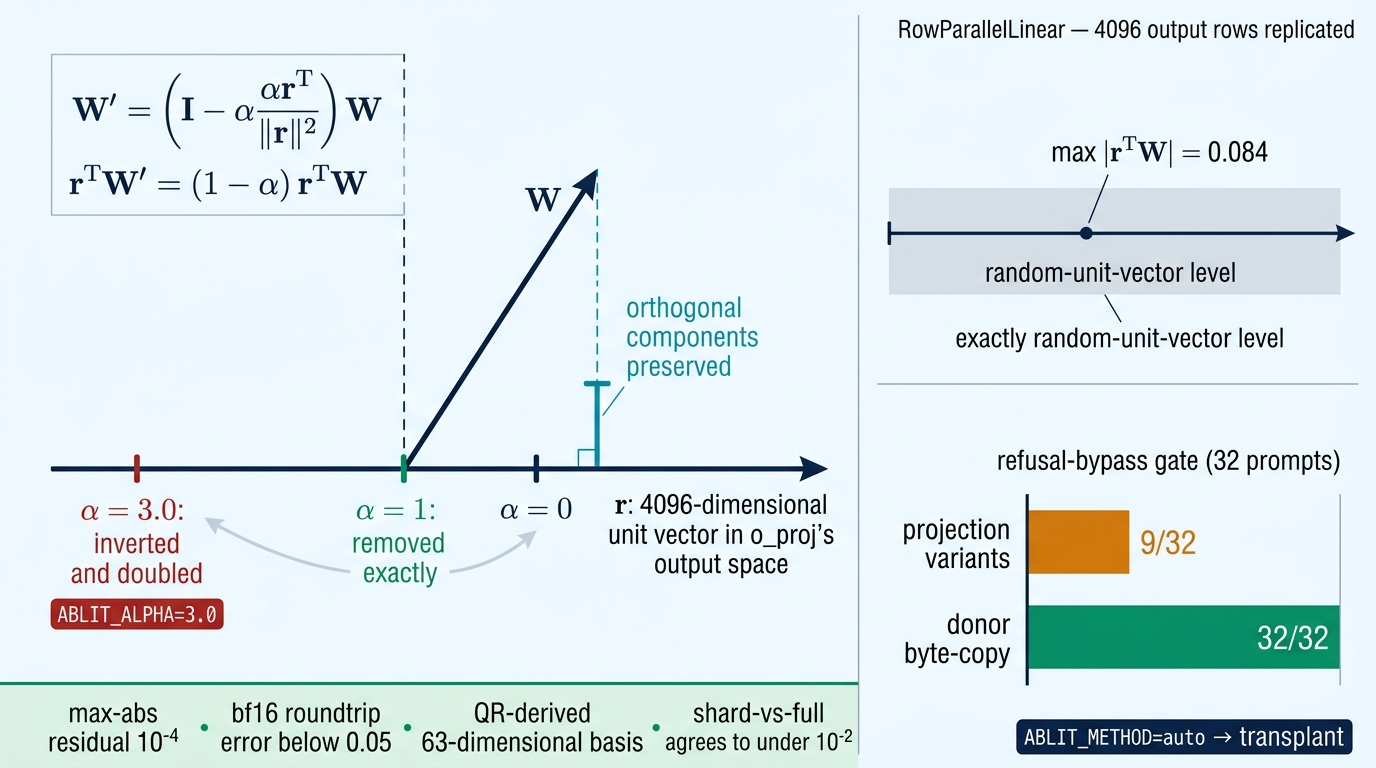
\includegraphics[width=\textwidth]{figures/ch17-projection-retired.png}
\caption{The elegant method, and the measurement that retired it. Classic
abliteration orthogonalizes each \code{o_proj} weight against a published
refusal direction $r$, so that
$r^{\top}W' = (1-\alpha)\,r^{\top}W$: at $\alpha=1$ the refusal component is
removed exactly, and at the published $\alpha=3.0$ it is inverted and doubled,
while components orthogonal to $r$ are untouched. The overlay's tests verify
all of that to unusual depth --- including that editing the full
$4096 \times 8192$ weight and editing two $4096 \times 4096$ column shards
independently agree to under $10^{-2}$, which is what makes a per-rank
load-time edit legal. What the lab then measured is the rest of the story: the
shipped directions' maximum $\lvert r^{\top}W\rvert$ against stock
\code{o_proj} was $0.084$, at random-unit-vector level. The publisher's
own projection variants top out at 9/32 on their refusal-bypass gate;
byte-copying the donor's weights scores 32/32.}
\label{fig:ablit-projection}
\end{figure}

\subsection{Byte-transplant: donor surgery with a manifest}

The mode that actually works, and the default when its tensors are present,
is \code{transplant}: byte-replace the stock \code{o_proj} weights of layers
15--45 --- 31 tensors, including the checkpoint's MTP block at layer 45 ---
with the corresponding tensors from an already-abliterated donor,
\code{dealignai/GLM-5.3-Flash-UNCENSORED-NVFP4}. This reproduces the
published \code{dealign-oproj-transplant} recipe
(\code{drowzeys/keys-GLM-5.3-Flash-NVFP4-ablit-l15-45-anchorstock}). The
trick that makes a cross-checkpoint transplant legal: this EXL3 checkpoint's
\code{o_proj} tensors are byte-identical to the NVFP4 body's --- native bf16
in both, same 120-shard layout --- so a donor tensor drops in exactly.
Layers 0--14 are deliberately left stock as \emph{safety anchors}
(\Cref{fig:transplant-map}); a stock early stack is part of the published
recipe, not an omission. Fidelity was checked against the published
fingerprint: mean relative delta $0.126$, with the layer-44 outlier measured
at $0.737$ against the published $0.74$.

Mechanically, each donor tensor arrives as a raw bf16 file
(\code{L15.bin} through \code{L45.bin}) plus a \repofile{MANIFEST.json} entry carrying shard, key, dtype,
shape, byte count, and per-tensor sha256. The runtime
(\repofile{overlay/ablit_runtime.py}) re-verifies hashes at load, checks
exact byte counts and BF16 dtype, and slices the donor's \emph{input}
dimension per TP rank --- \code{donor[:, rank*local_in:(rank+1)*local_in]}
after asserting \code{full_in == local_in * world} --- so each rank
transplants exactly its shard. The test suite proves the rank-0/rank-1
concatenation equals the donor byte-for-byte.

Two smaller checks carry real
scar tissue. A per-layer relative-$L_2$ delta must exceed $0.1$, guarding
against transplanting stock-identical tensors from a wrong donor revision.
And the donor buffer is explicitly moved to the weight's device, memorialized
in a comment --- ``proj path already does \code{r.to(weight.device)};
transplant forgot'' --- after a live-serve crash where the delta computation
mixed CPU and CUDA tensors. The DFlash2 drafter is never touched, but
\envvar{ABLIT_INCLUDE_MTP=1} transplants the MTP block's own
\code{o_proj}, because a stock MTP head keeps proposing refusals that the
edited target then rejects.

\begin{hblesson}
Every failure in the abliteration path is a hard \code{AblitError}: missing
manifest, missing tensors, missing direction file, bad layer range, shape
mismatch --- and, crucially, an enabled run that edits \emph{zero} layers
raises ``no o\_proj was edited'' rather than serving quietly. The runtime's
own phrase is the doctrine: \emph{fail loud beats silent stock weights}.
An operator who asked for an abliterated serve and got a stock one would
attribute the model's refusals to the method, publish a wrong conclusion,
and never see an error. This is \Cref{ch:patches}'s fail-closed patch
discipline applied to a new asset class: when the payload is weights, a
silent no-op is not a degraded mode --- it is a false experimental result.
\end{hblesson}

\begin{figure}[htbp]
\centering
\adjustbox{max width=\textwidth}{%
\begin{tikzpicture}
  % ---- layer strip: 0.28 cm per layer ----
  \node[hbtitle, anchor=south west] at (0,1.10)
    {o\_proj transplant map (LAYER\_MAP.json: 46 entries, hidden 4096)};
  % anchors 0-14 (15 layers)
  \draw[fill=lightgray!45, draw=hbSteel, thick] (0,0) rectangle (4.20,0.9);
  \node[font=\scriptsize, align=center] at (2.10,0.45)
    {layers 0--14\\safety-anchor (stock)};
  % edits 15-44 (30 layers)
  \draw[fill=hbAmber!30, draw=hbAmber!80!black, thick] (4.20,0) rectangle (12.60,0.9);
  \node[font=\scriptsize, align=center] at (8.40,0.45)
    {layers 15--44 --- role \emph{edit} (30 tensors, bf16 byte-copy)};
  % MTP 45
  \draw[fill=hbAccent!12, draw=hbAccent!70!black, thick] (12.60,0) rectangle (13.30,0.9);
  \node[font=\tiny, align=center] at (12.95,0.45) {45\\MTP};
  % boundary labels
  \node[hblabel, anchor=north] at (4.20,-0.05) {15};
  \node[hblabel, anchor=north] at (12.60,-0.05) {45};
  % arrow from edit region to slicing
  \draw[hbflow] (8.40,-0.15) -- (8.40,-1.02)
    node[hblabel, midway, right=1.5mm, align=left]
    {end of load\_weights,\\before CUDA-graph capture};
  % ---- per-rank slicing ----
  \node[hbtitle, anchor=south west] at (0,-1.45)
    {per-rank slice at load};
  \node[hblabel, anchor=south west] at (4.1,-1.45)
    {(input dim sharded; 4096 rows replicated)};
  \draw[fill=hbBlue!8, draw=hbSteel, thick] (0,-2.9) rectangle (4.5,-1.6);
  \node[font=\scriptsize, align=center] at (2.25,-2.25)
    {donor[:, 0:in/2]\\$\rightarrow$ rank 0};
  \draw[fill=hbBlue!8, draw=hbSteel, thick] (4.5,-2.9) rectangle (9.0,-1.6);
  \node[font=\scriptsize, align=center] at (6.75,-2.25)
    {donor[:, in/2:in]\\$\rightarrow$ rank 1};
  \draw[decorate,decoration={brace,amplitude=4pt,mirror}, thick, color=hbSteel]
    (0,-3.05) -- (9.0,-3.05)
    node[hblabel, midway, below=5pt]
    {rank 0 $\Vert$ rank 1 $=$ donor, byte-exact (tested at layers 16, 20, 31, 44)};
  \coordinate (manref) at (9.0,-2.25);
  \node[hbpatch, right=8mm of manref, align=left, font=\scriptsize] (man)
    {MANIFEST.json:\\shard, key, dtype,\\shape, nbytes, sha256\\--- re-verified at load};
  \draw[hbarrow, dashed] (man.west) -- (manref);
\end{tikzpicture}%
}
\caption{The transplant map. Layers 0--14 stay stock as safety anchors;
layers 15--45 (including the MTP block) have their bf16 \code{o_proj}
tensors byte-replaced with donor weights, sliced per TP rank along the input
dimension and verified against per-tensor sha256 manifests. The on-disk EXL3
checkpoint is never modified.}
\label{fig:transplant-map}
\end{figure}

\begin{table}[htbp]
\centering\small
\caption{The three abliteration knobs the prose discusses
(\repofile{.env.example} documents the full surface; all knobs are inert
unless \envvar{ABLIT} is exactly \code{1}).}
\label{tab:ablit-knobs}
\begin{tabular}{ll>{\raggedright\arraybackslash}p{6.4cm}}
\toprule
Knob & Default & Effect \\
\midrule
\envvar{ABLIT} & 0 & master gate; any value but \code{1} is stock \\
\envvar{ABLIT_METHOD} & auto & \code{transplant} when donor tensors are
present, else \code{proj} \\
\envvar{ABLIT_ALPHA} & 3.0 & $\alpha$ in the projection formula; 1.0 is pure
removal, 3.0 the published over-projection \\
\bottomrule
\end{tabular}
\end{table}

\section{Fetching 2.7\,GiB instead of 164\,GiB}

The donor is a full 320B-class checkpoint: roughly 164\,GiB across 120
safetensors shards. The transplant needs 31 tensors out of it.
\repofile{ablit/fetch_transplant.py} refuses to pay for the difference: it
pulls \emph{only the \code{o_proj} byte ranges} over HTTP Range requests ---
about 2.7\,GiB total --- and never materializes the donor checkpoint at all
(\Cref{fig:range-fetch}).

The flow is a small exercise in trusting the right source. The fetcher reads
\repofile{LAYER_MAP.json} and selects the layers whose role is \code{edit}
or \code{mtp-edit}; but for shard placement it fetches the donor's own
\repofile{model.safetensors.index.json} weight map. Where the two
disagree it prints a note and uses the donor index --- the map is a hint,
the donor is truth. Per layer it then reads the shard's first 8 bytes (the
safetensors header length), fetches the JSON header, looks up the tensor's
\code{data_offsets}, and issues a range request for exactly those bytes.
Transfers run in 8\,MiB chunks with 4 retries under a linear backoff of
$3\times\text{attempt}$ seconds, and resume \emph{within} a partially
fetched range. Each tensor is written via a \code{.tmp} file and atomic
rename, and \repofile{MANIFEST.json} is updated after \emph{every} tensor.
An interrupted fetch therefore loses at most one tensor's progress, and a
rerun skips any file whose sha256 already matches the manifest. The final line
reports \code{ok/31 tensors} and the gigabytes actually moved. The manifest
this produces is the same one the runtime verifies at load: the fetch tool
and the serve share one contract, keyed by hash.

Nothing in that flow is specific to abliteration. A safetensors shard carries
a JSON header naming every tensor's byte offsets, so any checkpoint served by
a host that honours Range requests is randomly addressable at tensor
granularity --- which is what turns ``31 tensors out of 120 shards'' from a
164\,GiB download into a 2.7\,GiB one.

\begin{figure}[htbp]
\centering
\adjustbox{max width=\textwidth}{%
\begin{tikzpicture}[node distance=7mm and 12mm]
  % donor shard stack
  \node[hbfaint, minimum width=32mm, align=center] (s1)
    {model-00001-of-00120\\.safetensors};
  \node[hbfaint, below=2.5mm of s1, minimum width=32mm, align=center] (s2)
    {model-00029-of-00120\\(holds an o\_proj)};
  \node[hbfaint, below=2.5mm of s2, minimum width=32mm, align=center] (s3)
    {\vdots};
  \node[hbfaint, below=2.5mm of s3, minimum width=32mm, align=center] (s4)
    {model-00120-of-00120};
  \begin{scope}[on background layer]
    \node[hbgroup, fit=(s1)(s4),
      label={[hbtitle]above:donor: 120 shards, \(\approx\)164\,GiB}] (donor) {};
  \end{scope}
  % header pipeline
  \node[hbbox, right=20mm of s2, align=left, font=\scriptsize] (hdr)
    {1. read first 8 B (header length)\\
     2. fetch JSON header\\
     3. data\_offsets[key] $\rightarrow$ [a, b)\\
     4. Range: bytes=8+n+a .. 8+n+b-1};
  \draw[hbflow] (donor.east |- hdr.west) -- (hdr.west)
    node[hblabel, midway, above=1mm] {per tensor};
  % output
  \node[hbgpu, right=26mm of hdr, align=center] (out)
    {ablit/transplant/\\L15.bin \ldots{} L45.bin\\31 tensors, \(\approx\)2.7\,GiB};
  \node[hbpatch, below=5mm of out, align=center, font=\scriptsize] (mani)
    {MANIFEST.json\\updated after every tensor\\sha256 per file};
  \draw[hbflow] (hdr) -- (out)
    node[hblabel, midway, above=1mm, align=center, font=\tiny]
    {8\,MiB chunks \(\cdot\) 4 retries\\.tmp + atomic rename};
  \draw[hbarrow, <->] (out) -- (mani)
    node[hblabel, midway, right=1mm] {resume: matching hash $\Rightarrow$ skip};
  % authority note
  \node[hblabel, below=4mm of hdr, align=center]
    {shard placement from the donor's own index.json ---\\
     LAYER\_MAP.json is a hint, the donor is truth};
\end{tikzpicture}%
}
\caption{Surgical fetching: HTTP Range requests extract the 31 \code{o_proj}
tensors (about 2.7\,GiB) from the donor's 120 shards (about 164\,GiB)
without ever downloading a shard. Every tensor is hash-manifested as it
lands, making the fetch resumable per tensor and the manifest the shared
contract between fetcher and runtime.}
\label{fig:range-fetch}
\end{figure}

\section{Honest scaling: a launcher for hardware the lab does not own}

The transplant scoped every claim to a hash it could verify; the chapter's
second subject faces the same test with no evidence to offer at all.
\Cref{ch:scaling} showed the DeepSeek recipe scaling to a third Spark with
measurements in hand. The GLM repository faces the same demand --- users with four
GB10s asked for TP=4 --- from a weaker position: the lab has no 4-Spark kit.
Its answer, merged as PR \ghissue{105} on the GLM tracker, is
\repofile{start-tp4.sh}: a roughly 90\,\% structural clone of
\repofile{start.sh} whose header says exactly what it is ---
``\textsc{experimental} \ldots{} Optional sibling of start.sh. Does not
change the supported 2$\times$ TP=2 path. \emph{Untested here (no 4-Spark
kit).} A user with four GB10s can try.'' The claim is scoped to what was
verified: the script's structure, not its behavior on real hardware.

The interesting engineering is in how the untested path is \emph{isolated}
from the tested one. The launcher sources \repofile{.env} and then layers
\repofile{.env.tp4} on top (auto-copied from \repofile{.env.tp4.example} on
first run, and git-ignored). The overlay wins over the two-node knobs, and
\repofile{start.sh} never reads the file --- so a four-node experiment
cannot leak a single variable into the supported lane. Container names are
namespaced the same way: \code{glm53-exl3-tp4-head} and \code{-w1/-w2/-w3},
``so a TP=2 serve is not accidentally reused.'' The corollary is spelled
out too: \code{./start.sh stop} does not know about ranks 2/3 --- each
topology owns its own stop path. The rest is generalization plumbing:
per-rank \envvar{WORKER2_*} / \envvar{WORKER3_*} variable families
defaulting to the rank-1 values, a rank-switch helper family behind every
SSH, cache, and NIC pin, a preflight that loops all three workers, and even
a deliberately preserved dead-code heredoc so a \code{diff} against
\repofile{start.sh} stays legible. Notably, no scheduler or KV retuning is
attempted: the same
\envvar{GPU_MEM_UTIL=0.87}, \code{MNBT} 7168, and \code{max_num_seqs} 4
ride along, because inventing tuned numbers for unmeasured hardware would
be exactly the kind of claim this repository refuses to make.

The price of that isolation is duplication: a second launcher that is roughly
90\,\% a clone of the first, kept diff-legible on purpose down to a preserved
dead-code heredoc. That is the trade being made --- redundancy in the
repository in exchange for a supported lane a four-node experiment cannot
reach (\Cref{fig:tp4-containment}).

\begin{figure}[htbp]
\centering
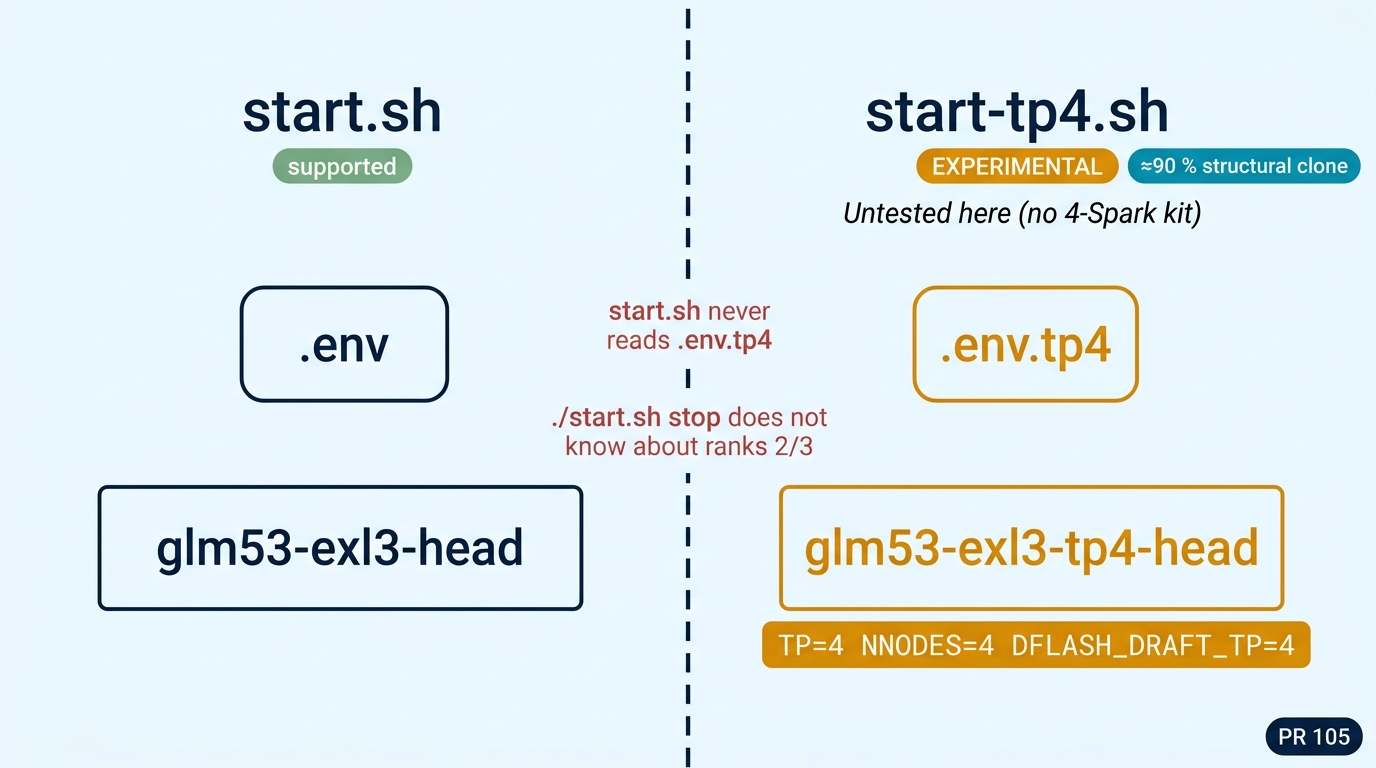
\includegraphics[width=\textwidth]{figures/ch17-tp4-containment.png}
\caption{Shipping a configuration you cannot test. \repofile{start-tp4.sh}
(PR \ghissue{105}) is roughly a 90\,\% structural clone of
\repofile{start.sh}, and the engineering is in the barrier rather than the
clone: both lanes read \repofile{.env}, but only the TP=4 launcher layers
\repofile{.env.tp4} on top --- \repofile{start.sh} never reads that file, so a
four-node experiment cannot leak a single variable into the supported lane.
Container names are namespaced the same way, and each topology owns its own
stop path, because \code{./start.sh stop} does not know about ranks 2/3. No
scheduler or KV retuning rides along: \envvar{GPU_MEM_UTIL=0.87}, MNBT 7168
and \code{max_num_seqs} 4 are unchanged, because inventing tuned numbers for
unmeasured hardware would be exactly the kind of claim this repository refuses to
make. The price is duplication, kept diff-legible on purpose down to a
preserved dead-code heredoc.}
\label{fig:tp4-containment}
\end{figure}

\begin{lstlisting}[language=bash]
# .env.tp4 -- layered over .env by start-tp4.sh ONLY (start.sh never reads it)
TP=4  NNODES=4  DFLASH_DRAFT_TP=4     # shard the drafter across all four ranks
NCCL_CROSS_NIC=1                      # ring/switch fabric, not one direct cable
WORKER2_IP=10.0.0.3  WORKER3_IP=10.0.0.4
HEAD_CX7_IB=rocep1s0f0,rocep1s0f1     # dual-port ring: both CX7 HCAs, comma list
CONTAINER_HEAD=glm53-exl3-tp4-head    # ... -w1 -w2 -w3: a TP=2 serve
                                      # can never be reused by accident
\end{lstlisting}

\begin{table}[htbp]
\centering\small
\caption{What the \repofile{.env.tp4} overlay changes relative to the
supported two-node lane.}
\label{tab:tp4-deltas}
\begin{tabular}{>{\raggedright\arraybackslash}p{3.4cm}>{\raggedright\arraybackslash}p{3.3cm}>{\raggedright\arraybackslash}p{5.6cm}}
\toprule
Knob & TP=2 (supported) & TP=4 (experimental) \\
\midrule
\envvar{TP} / \envvar{NNODES} & 2 / 2 & 4 / 4 \\
\envvar{DFLASH_DRAFT_TP} & 2 & 4 (drafter sharded across all ranks) \\
\envvar{NCCL_CROSS_NIC} & 0 (one direct QSFP cable) & 1 (ring or switch among
all ranks) \\
Worker set & \envvar{WORKER_*} only & adds \envvar{WORKER2_*} /
\envvar{WORKER3_*} (10.0.0.3 / 10.0.0.4), defaults mirroring rank 1 \\
HCA pins & one HCA per node & comma-separated dual-port lists supported;
\code{_tp4_first_ib} picks the first for GID preflight \\
Containers & \code{glm53-exl3-head} / \code{-worker} &
\code{glm53-exl3-tp4-head} / \code{-w1/-w2/-w3}; own \code{stop} and
per-rank \code{logs 1|2|3} \\
Scheduler / KV tuning & measured keeps & unchanged --- no invented numbers
for unmeasured hardware \\
\bottomrule
\end{tabular}
\end{table}

The contrast with \Cref{ch:scaling} is worth one paragraph, because the two
labs hit different walls. DeepSeek-V4-Flash's TP=3 required eleven anchored
model-code edits, a padded attention geometry, and a warring pair of pad
resolutions before a third rank could even boot --- and then shipped with a
measured ledger of what three nodes buy and cost. GLM-5.3-Flash's TP=4 is,
architecturally, ``purely more ranks'': no divisibility wall, no pad, the
same vLLM flags. What it lacks is evidence, and the repository treats missing
evidence exactly as \Cref{ch:scaling}'s repository treated numerics risk: give
the risky topology its own launcher, its own env file, its own container
namespace, and its own stop path, so the experiment cannot contaminate the
production lane. And label the untested part untested, in the header,
where a user reads it before running anything. The earlier prefill study
had already set expectations in the same spirit: TP=4 is ``not
$\sim$2$\times$, different topology, and this is a 2-node recipe.''

\begin{hbnote}
\textbf{What the next edition owes this section.} The four-Spark lane is the
one place this book documents a configuration nobody has run. When a
four-node kit exists it will get the treatment \Cref{ch:scaling} gave the
third Spark --- one knob per boot, a dated ledger, a fabric census, and a
verdict that may well be negative. The question is already sharp. Adding a
third node cut the bytes each rank must stream to $\approx$11.5\,GB and the
streaming model priced the step at $\approx$48\,ms; measured decode came
out at 64.3 \tokspersec{}, no faster than two nodes, because fixed per-step
cost ate the entire bandwidth gain (\Cref{ch:perf}). A fourth node inherits
that arithmetic and adds collectives on top of it. Whether the curve bends
or flattens again is not derivable from the byte model. It has to be
measured --- and until it is, this section is the honest end of the story.
\end{hbnote}

\section{The fabric truths a fourth Spark rests on}

Whether at two nodes or four, every rank of this deployment stands on a
stack of RoCEv2 facts that were learned the hard way and then promoted into
preflight code. \Cref{ch:fabric} covered the DeepSeek pair's fabric; the GLM
repository's contribution is the \emph{GID index} lore, and it generalizes to any
multi-NIC RDMA cluster.

A RoCE GID table maps small integer indices to addresses, per NIC, per
node --- and nothing guarantees two nodes agree. On the second GLM kit
(GLM tracker \ghissue{26}, contributed by im0xMagnus), the RoCE-v2
\code{::ffff:<ip>} entry sat at index 4 on the head and index 3 on the
worker; the only index the two nodes had in common (2) was a RoCE-v1 entry,
which cannot serve a fabric pinned to \envvar{NCCL_IB_ROCE_VERSION_NUM=2}.
No single shared \envvar{NCCL_IB_GID_INDEX} could ever work on that pair
--- the knob's very shape was wrong. The fix is per-rank GID pins
(\envvar{HEAD_GID} / \envvar{WORKER_GID}, defaulting to the shared index 3),
extended to \envvar{WORKER2_GID} / \envvar{WORKER3_GID} in the TP=4 overlay
(\Cref{fig:gid-mismatch}).

\begin{hbwarstory}
The nastier failure mode arrived first, as GLM tracker \ghissue{16}
(Jim Bisesi, from an independent second-kit reproduction): an
\emph{all-zero} GID entry. An empty entry passes every earlier network
check --- links up, pings fine, NCCL initializes --- and then kills its
rank roughly 60 seconds into the boot with \code{ibv_modify_qp} errno 61,
``No data available,'' deep in queue-pair state transition. By that point
any operator has long stopped watching for network errors. The launcher's
preflight now validates that each rank's GID index names a \emph{populated}
entry in that rank's own
\repofile{/sys/class/infiniband/<dev>/ports/1/gids/<idx>}. On refusal it
dumps both nodes' full 0--7 GID tables with their RoCE v1/v2 types and the
selection rule: pick each node's \code{::ffff:<ip>} entry whose type is
RoCE v2; the two indices need not match.
\end{hbwarstory}

The same promotion-to-preflight pattern covers the sub-gigabyte memory
margin: \envvar{GPU_MEM_UTIL=0.87} requires at least 105.9\,GiB free, and
nodes with resident desktop services miss that bar by under a gigabyte. The
README encodes the documented fallback pair rather than leaving the
operator to rediscover the margin from an OOM at minute forty of a weight
load. The
through-line of all three: a fact that once cost a debugging session ---
a v2 entry at different indices, an all-zero GID, a sub-gigabyte memory
margin --- is worth a preflight check that costs milliseconds, dumps its
evidence when it refuses, and turns a mid-boot rank death into a launcher
error with a remedy attached.

\begin{figure}[htbp]
\centering
\adjustbox{max width=\textwidth}{%
\begin{tikzpicture}[node distance=8mm and 16mm]
  % head GID table
  \node[hbhost, minimum width=46mm, align=left, font=\scriptsize] (head)
    {\textbf{head} --- rocep1s0f1, GID table\\[1mm]
     idx 2: fe80::\ldots{} \hfill RoCE v1\\
     idx 3: 0000:0000:\ldots:0000 \hfill \textcolor{hbAccent}{all-zero}\\
     idx 4: ::ffff:$\langle$head-ip$\rangle$ \hfill \textbf{RoCE v2}};
  % worker GID table
  \node[hbhost, right=24mm of head, minimum width=46mm, align=left, font=\scriptsize] (wrk)
    {\textbf{worker} --- rocep1s0f0, GID table\\[1mm]
     idx 2: fe80::\ldots{} \hfill RoCE v1\\
     idx 3: ::ffff:$\langle$worker-ip$\rangle$ \hfill \textbf{RoCE v2}\\
     idx 4: (empty)};
  % shared-index attempt (fails)
  \node[hbwarn, below=11mm of $(head.south)!0.5!(wrk.south)$,
        align=center, font=\scriptsize] (shared)
    {one shared NCCL\_IB\_GID\_INDEX?\\only common index (2) is RoCE v1\\
     $\Rightarrow$ cannot serve a v2 fabric};
  \draw[hbfail] (head.south) -- (shared.north west);
  \draw[hbfail] (wrk.south) -- (shared.north east);
  % per-rank pins (works)
  \node[hbgpu, below=8mm of shared, align=center, font=\scriptsize] (pins)
    {per-rank pins: HEAD\_GID=4, WORKER\_GID=3\\
     (TP=4 adds WORKER2\_GID / WORKER3\_GID)};
  \draw[hbok] (shared) -- (pins)
    node[hblabel, midway, right=1mm] {\ghissue{26}};
  % preflight annotation
  \node[hbpatch, right=10mm of pins, align=left, font=\scriptsize] (pf)
    {preflight (\ghissue{16}): index must name a\\
     populated entry on that rank's OWN NIC;\\
     refusal dumps both GID tables 0--7.\\
     All-zero entry: passes every check,\\
     kills the rank \(\approx\)60\,s in ---\\
     ibv\_modify\_qp errno 61};
  \draw[hbarrow, dashed] (pf.west) -- (pins.east);
\end{tikzpicture}%
}
\caption{Why the GID index is per-NIC state, not cluster configuration. On
the second GLM kit the RoCE-v2 entry sat at index 4 on the head and 3 on
the worker, the only common index was v1, and an all-zero entry passed
every network check before killing its rank a minute into boot. The
launcher validates each rank against its own device and prints the
evidence when it refuses.}
\label{fig:gid-mismatch}
\end{figure}

\section{The open lab}

Preflight checks are how the lab encodes its lessons for machines; its last
subject is how it encodes them for people. Everything in Part II so far --- the quantized bet, the drafter, the
proof-carrying patches, the transplants --- was built in ten days, in
public, by more than a dozen people. The repository's history (125 commits,
2026-08-26 through 2026-09-05) reads less like a solo project than like a
functioning lab with a door open: twelve named community contributors
landed substantive changes, and they cluster into three kinds of work.
Bring-up and hardening: Chris Scott's seed SM120 overlay (the repository's
literal first commit), Raymond Lucke's day-two template fix, Jim Bisesi's
GID preflight, Daniel Banu's env-only API auth, hecisaza's numeric-knob
validation, and Tutanka01's bring-up robustness work. Measurement, client,
and template infrastructure: Tutanka01's prefix-cache bench, Jenpo's
bounded Pi client configs, sovereignbrah's reasoning-effort prefix-cache
fix, and knapcio's XGrammar backports. Kernels and rightsizing:
plotarmordev's E2 kernel diagnostics and spinwait sweep, nood-co1's
indexer-workspace rightsizing, and im0xMagnus's \envvar{CG_ESTIMATE}
opt-out and per-rank-GID work.

The indexer-workspace rightsizing alone came to 1{,}743
lines --- of which 819 were tests. By September 1 the maintainership itself had
broadened: community PRs were being merged by netrunner (plotarmordev), and
a GitHub Sponsors funding model sat alongside the code. AI co-authorship is
carried openly rather than laundered: Cursor trailers on nearly all
maintainer commits, Claude Opus 5 on three community PRs, Claude Fable 5 on
two more, and two commits linking their full \code{Claude-Session} URLs.
The provenance of machine assistance is treated like any other provenance,
recorded where posterity can audit it.

What makes this durable is that the evidence culture is \emph{encoded in
the contribution machinery}, not left to the maintainer's taste. The issue
forms (PR \ghissue{126} on the GLM tracker, ported from the lab's Qwen3.8
kit) disable blank issues, enumerate the kit's actual knob surface in the
bug form's environment section, and pre-list the four most common
self-serve culprits --- incomplete weights, a slow-decode checklist keyed
to boot-log facts, the do-not-reduce-\envvar{MAX_MODEL_LEN} trap, and the
vision-request shape --- so a report arrives triaged. The improvement form
asks for measured before/after numbers.

The PR template goes further: a
contributor must say which knob, default, overlay, or kernel path changes
and the expected direction of any measured number; explain why the change
is safe on \emph{both} nodes of the two-node TP=2 lane; and show testing
that means something. In practice that is \code{bash -n} for scripts, an actual
cluster boot with boot-log facts, measured numbers in the README's own
format (median-of-5 \repofile{tests/bench_decode.py}, the cold-prefill
table), and, for any change touching the drafter, ``an acceptance
measurement, not just tok/s.'' That last clause is a whole chapter of speculative-decoding
doctrine compressed into a form field: throughput without acceptance is
exactly the number that lies (\Cref{ch:measurement}).

\begin{hbnote}
The governance even retracts. PR \ghissue{55} on the GLM tracker --- filed,
fittingly, via a Pi agent running against this very serve --- corrected the
credits. An incorrect abliteration-donor line and a contributor credit
added hours earlier the same day were dropped as ``not accurate,'' while the
genuine drowzeys recipe attribution stayed. Attribution held to the same
standard as benchmarks --- dated, checked, and publicly corrected when
wrong --- is the social mirror of Part I's measurement retractions
(\Cref{ch:lessons}): the lab versions its beliefs about \emph{people} the
way it versions its beliefs about numbers.
\end{hbnote}

\FloatBarrier

The three subjects of this chapter look unrelated until you notice they
fail in the same place. A served checkpoint is not a fixed artifact --- it
is bytes in memory that a load-time hook may lawfully rewrite, provided a
hash says which bytes and a hard error fires when none were touched. A
topology the lab cannot boot is not unsupported --- it is a claim with no
evidence behind it, shippable only inside its own launcher, its own env
file, and its own label. And a repository with a dozen hands in it is not a
governance problem but an evidence problem, solved with issue forms and PR
fields rather than with a maintainer's taste. In all three the discipline
is identical: scope the claim to what was verified, and make the boundary
where verification stops loud enough that nobody walks past it.

\section*{Takeaways}

\begin{itemize}
\item Excluding \code{o_proj} from quantization bought a capability months
early --- bf16 weights can be edited at load time, per TP rank, with the
pinned checkpoint untouched --- and measuring the method before shipping it
is what decided which edit. The published refusal directions proved
statistically random against stock \code{o_proj}, a maximum
$\lvert r^{\top}W\rvert$ of $0.084$ and 9/32 on the refusal-bypass gate, so
the recipe byte-transplants donor weights instead, at 32/32.
\item When the payload is weights, a silent no-op is a false experimental
result: every abliteration failure is a hard \code{AblitError}, and an
enabled run that edits zero layers raises. The integrity contract is a
sha256 manifest shared by fetcher and runtime --- which is also what turns
31 tensors out of 120 shards into a 2.7\,GiB HTTP Range fetch, resumable
per tensor, rather than a 164\,GiB download.
\item Honest scaling for hardware you lack means isolation plus a label:
an untested lane with its own launcher, env file, containers, and stop
path --- and no invented numbers.
\item Fabric identity is per-NIC state: GID indices need not match across
nodes, and the cure is per-rank pins plus a preflight that dumps its
evidence on refusal.
\item Governance can encode epistemics: triaged issue forms, a PR template
demanding acceptance measurements, open AI co-authorship, and credits
corrected in public.
\end{itemize}

\section{Two recipes, one method}

Set the two halves of this book side by side and almost every technical
decision diverges. Part I serves DeepSeek-V4-Flash from the vendor's own
native low-precision checkpoint; Part II bets on a community EXL3/TR3
4-bpw quant, mirrored for durability and defended by an independent KLD
panel. Part I's drafter is DSpark; Part II's is DFlash2, with its
candidate-selector lattice walk. Part I tunes and patches stock kernels;
Part II, when the fat-expert tax would not yield to configuration, wrote
its own CUDA and compiled it into the extension. One recipe reached a
third node with padded attention geometry and a measured ledger; the other
shipped a fourth-node launcher labeled untested. Even the failure modes
differ --- a starved scheduler knob here, a one-block circular slot map
there.

And yet an engineer who has read both halves will recognize that they are
the same book. Both recipes pin every artifact --- image digests, model
revisions, extension commits, patch anchors --- and refuse to run when the
bytes drift. Both apply every change fail-closed, so a fix that cannot
prove its target aborts the boot instead of serving a lie. Both measure
before believing: one knob per boot, dated receipts, noise bands,
acceptance alongside throughput, benchmarks that distrust themselves. And
both revert in public --- a withdrawn safety claim, a struck evidence
matrix, two prefill optimizations published as losses, a credit line
corrected by an agent using the very server it corrected. The bets were
opposite; the method was identical; and the method, not either bet, is
what produced two working frontier serving systems.

That is the thing to carry out of this book. The hardware on these desks
is unremarkable by datacenter standards --- two small machines and a
cable, twice over. What made a million tokens of context, speculative
decoding, vision, and tools run interactively on them was not a secret
kernel or a heroic all-nighter but a discipline applied without exception:
pin it, prove it, measure it, and say so out loud when you were wrong.
That discipline is not proprietary. It fits in a preflight check, a PR
template, a manifest, an issue form; it survives handover to new
maintainers and collaboration with machines; it worked twice, on opposite
bets, in the same small lab. Wherever your own frontier is --- whatever
model, whatever engine, whatever pair of machines --- it will work a third
time.
